\documentclass{cours}

\title{Géométrie dans l'Espace}

\begin{document}
    \maketitle{11}

    \begin{Gpartie}{Positions Relatives de Droites et de Plans} 
        \begin{Spartie}{Positions Relatives de Deux Plans} 
            Deux plans de l'espace non parallèles sont sécants. Leur intersection est une \emph{droite}.
            \begin{center}
                    \begin{minipage}{5cm}
\includegraphics[width=5cm]{rsc/11fig1a.png}\\ \centering Plans strictement parallèles\end{minipage}
                    \begin{minipage}{5cm}
\includegraphics[width=5cm]{rsc/11fig1b.png}\\ \centering Plans Confondus\phantom{p}\end{minipage} \\[2ex] % p pour alignement vertical 
                    C'est deux types de plans parallèles. \\
                    
\includegraphics[width=5cm]{rsc/11fig1c.png} \\
                    Plans sécants
                \parbox{\linewidth}{\captionof{figure}{\centering Illustration des Positions Relatives de Deux Plans}}
            \end{center}
            \begin{SSpartie}{Propriété} 
                Deux plans sont parallèles si et seulement si \emph{deux} droites \emph{sécantes} incluses dans le premier sont parallèles à deux droites sécantes dans le deuxième.
                \begin{center}
                        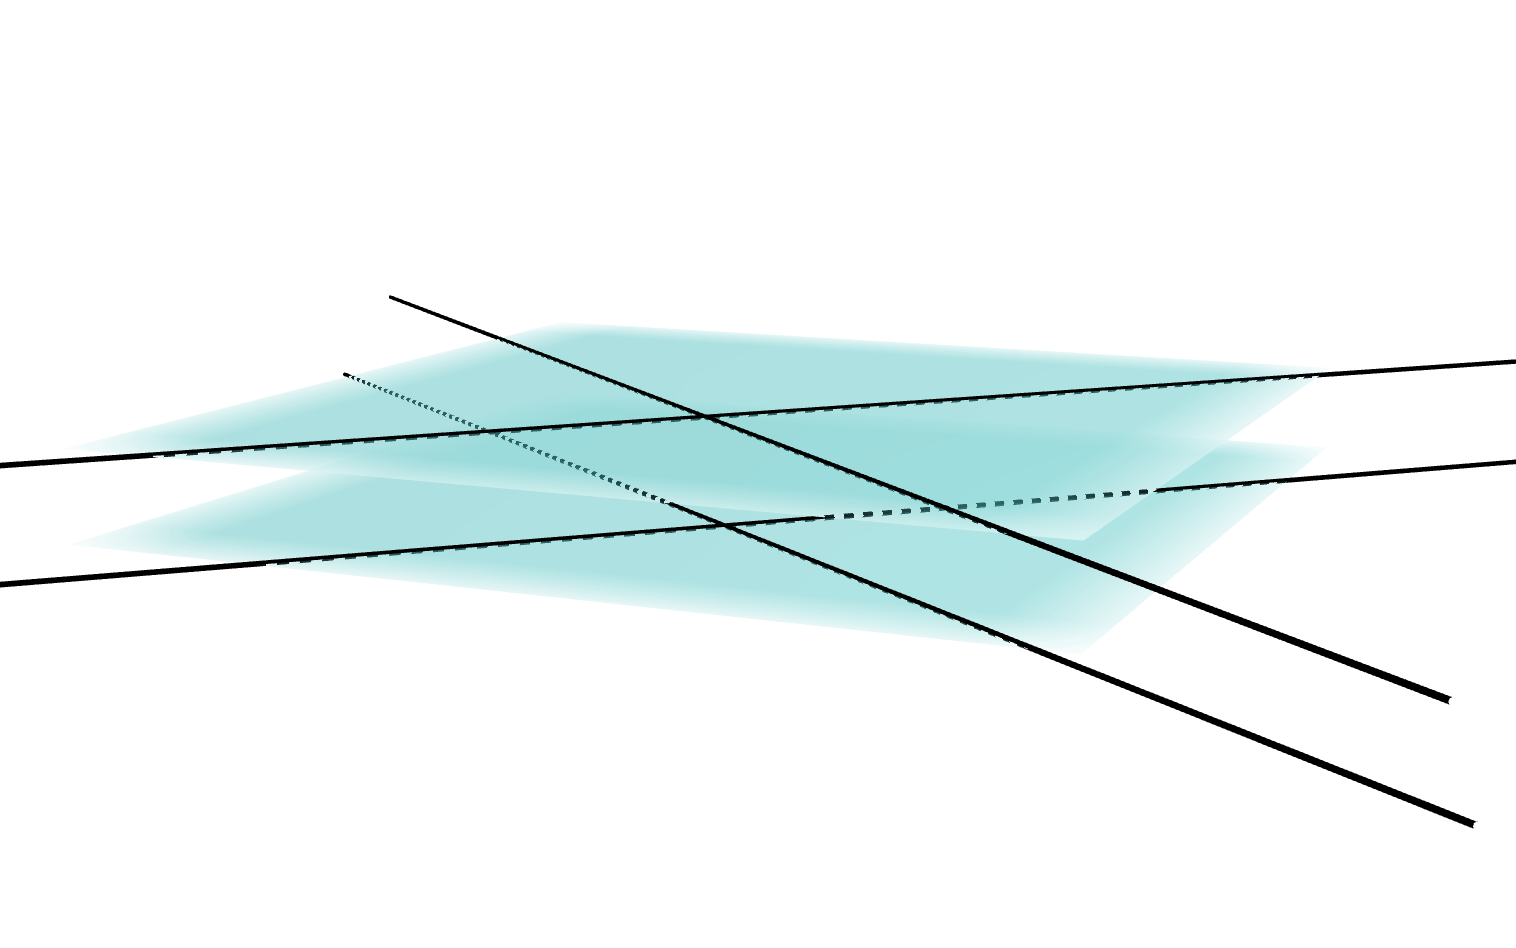
\includegraphics[width=5cm]{rsc/11fig2.png}
                    \parbox{\linewidth}{\captionof{figure}{\centering Illustration de la Propriété}}
                \end{center}
            \end{SSpartie}
            \pagebreak
            \begin{SSpartie}{Propriété} 
                Si deux plans sont parallèles, tout plan sécant à l'un est sécant à l'autre et les droites d'intersection sont parallèles.
                \begin{center}
                        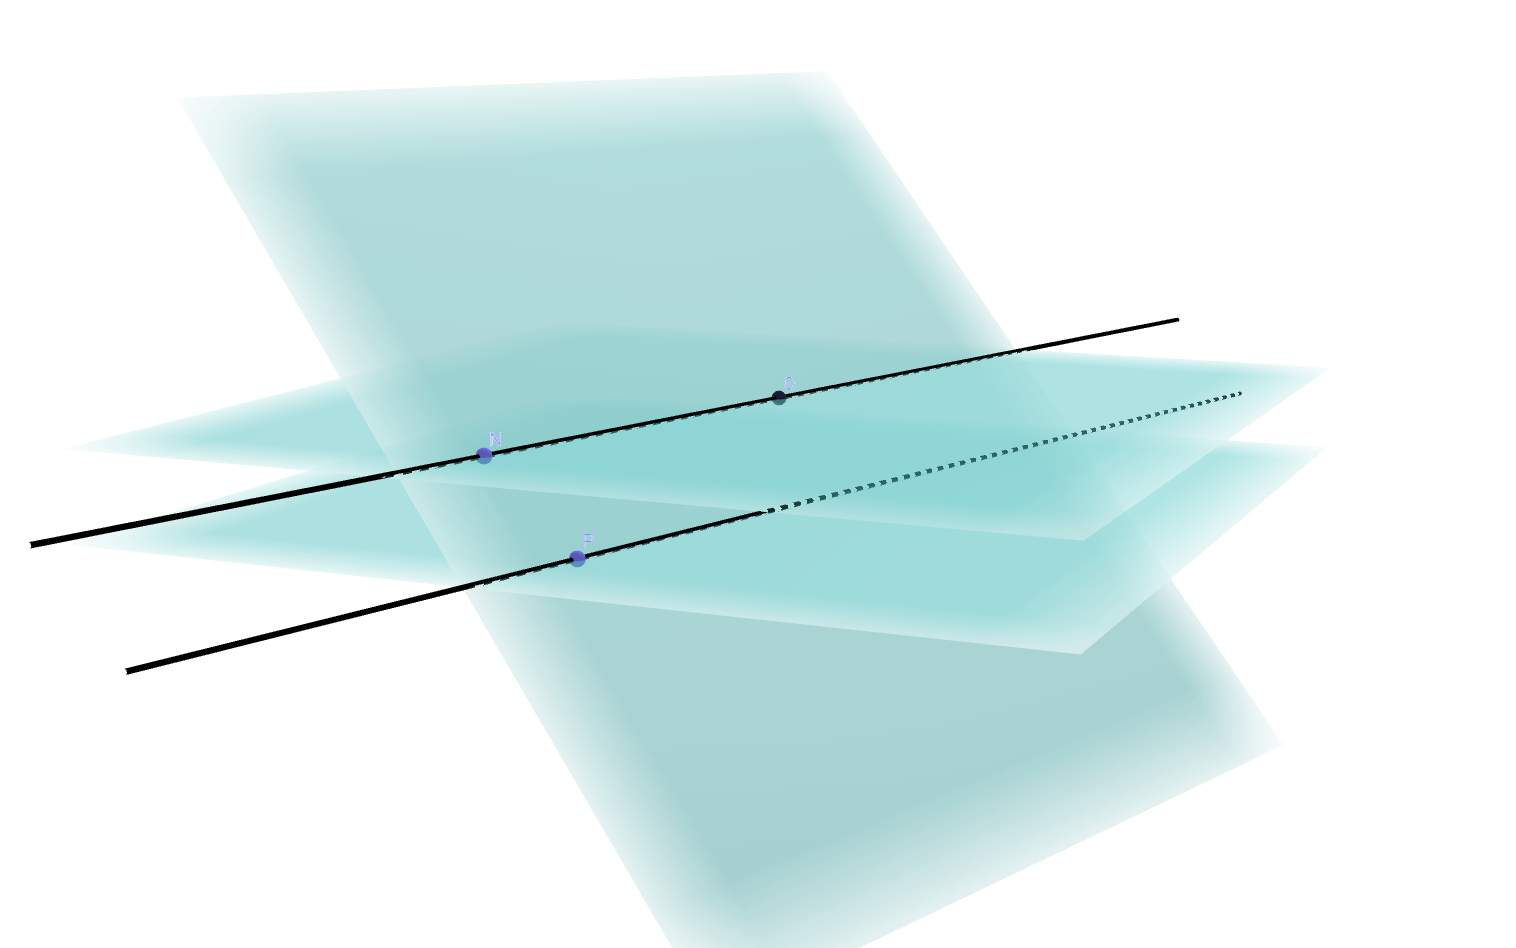
\includegraphics[width=5cm]{rsc/11fig3.png}
                    \parbox{\linewidth}{\captionof{figure}{\centering Illustration de la Propriété}}
                \end{center}
            \end{SSpartie}
            \begin{SSpartie}{Théorème dit ``du Toit''} 
                Si deux plans sécants $\mathcal{P}_1$ et $\mathcal{P}_2$ contiennent respectivement deux droites $d_1$ et $d_2$ parallèles, alors la droite d'intersection de $\mathcal{P}_1$ et $\mathcal{P}_2$ est parallèle à $d_1$ et $d_2$.
                \begin{center}
                        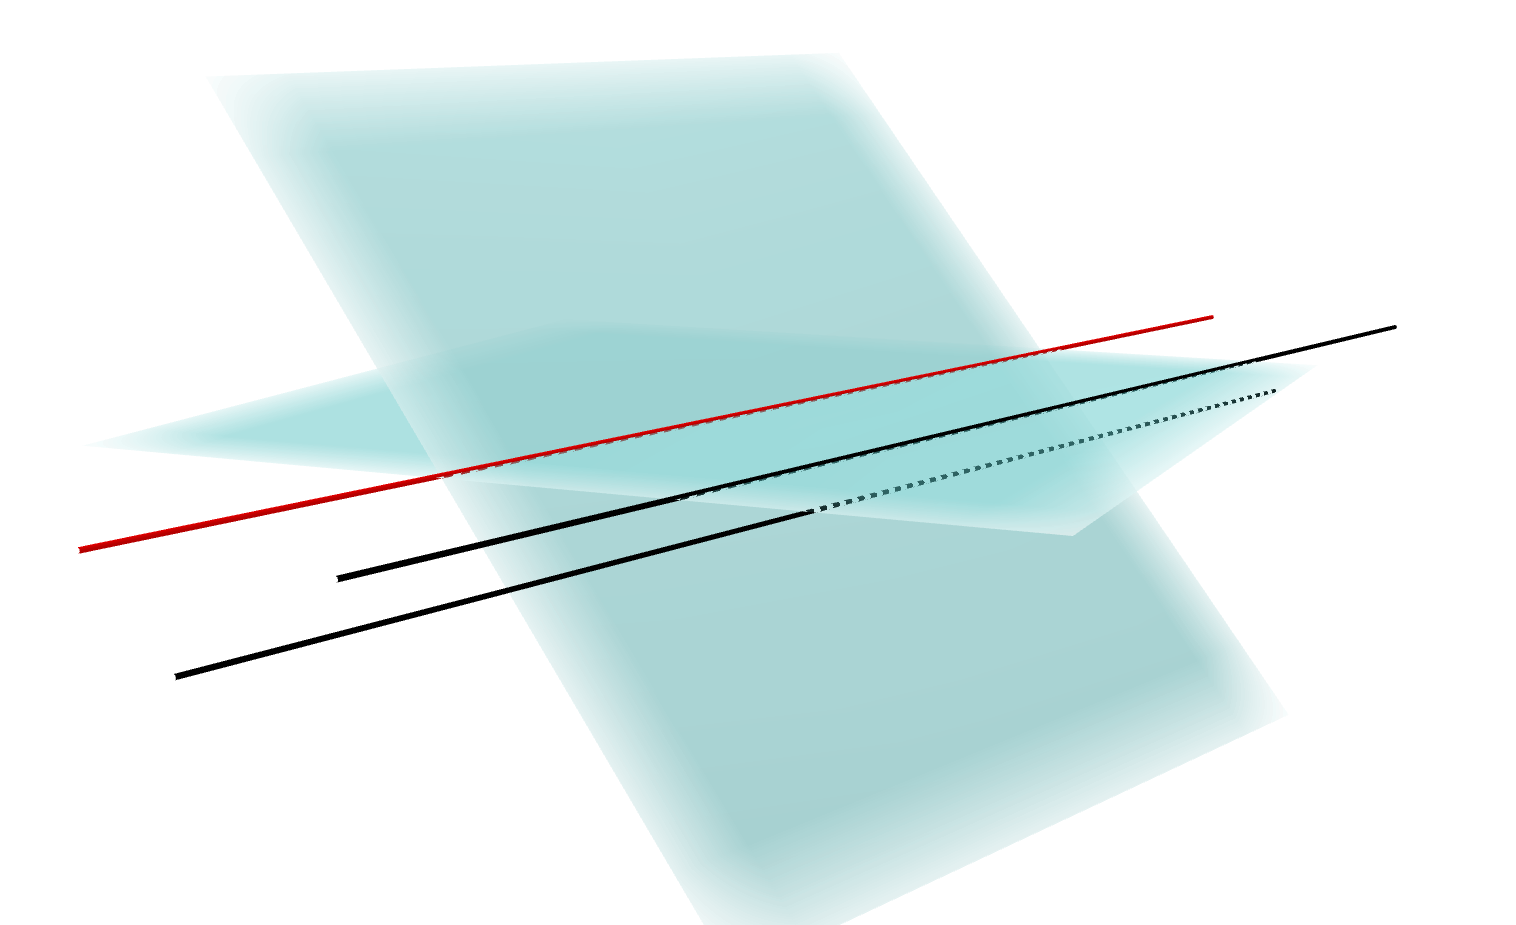
\includegraphics[width=5cm]{rsc/11fig4.png}
                    \parbox{\linewidth}{\captionof{figure}{\centering Illustration du Théorème}}
                \end{center}
            \end{SSpartie}
        \end{Spartie}
        \begin{Spartie}{Positions Relatives d'une Droite et un Plan} 
            Une droite non parallèle à un plan est sécante à ce plan. Leur intersection est un~\emph{point}.
            \begin{center}
                \begin{minipage}{4cm}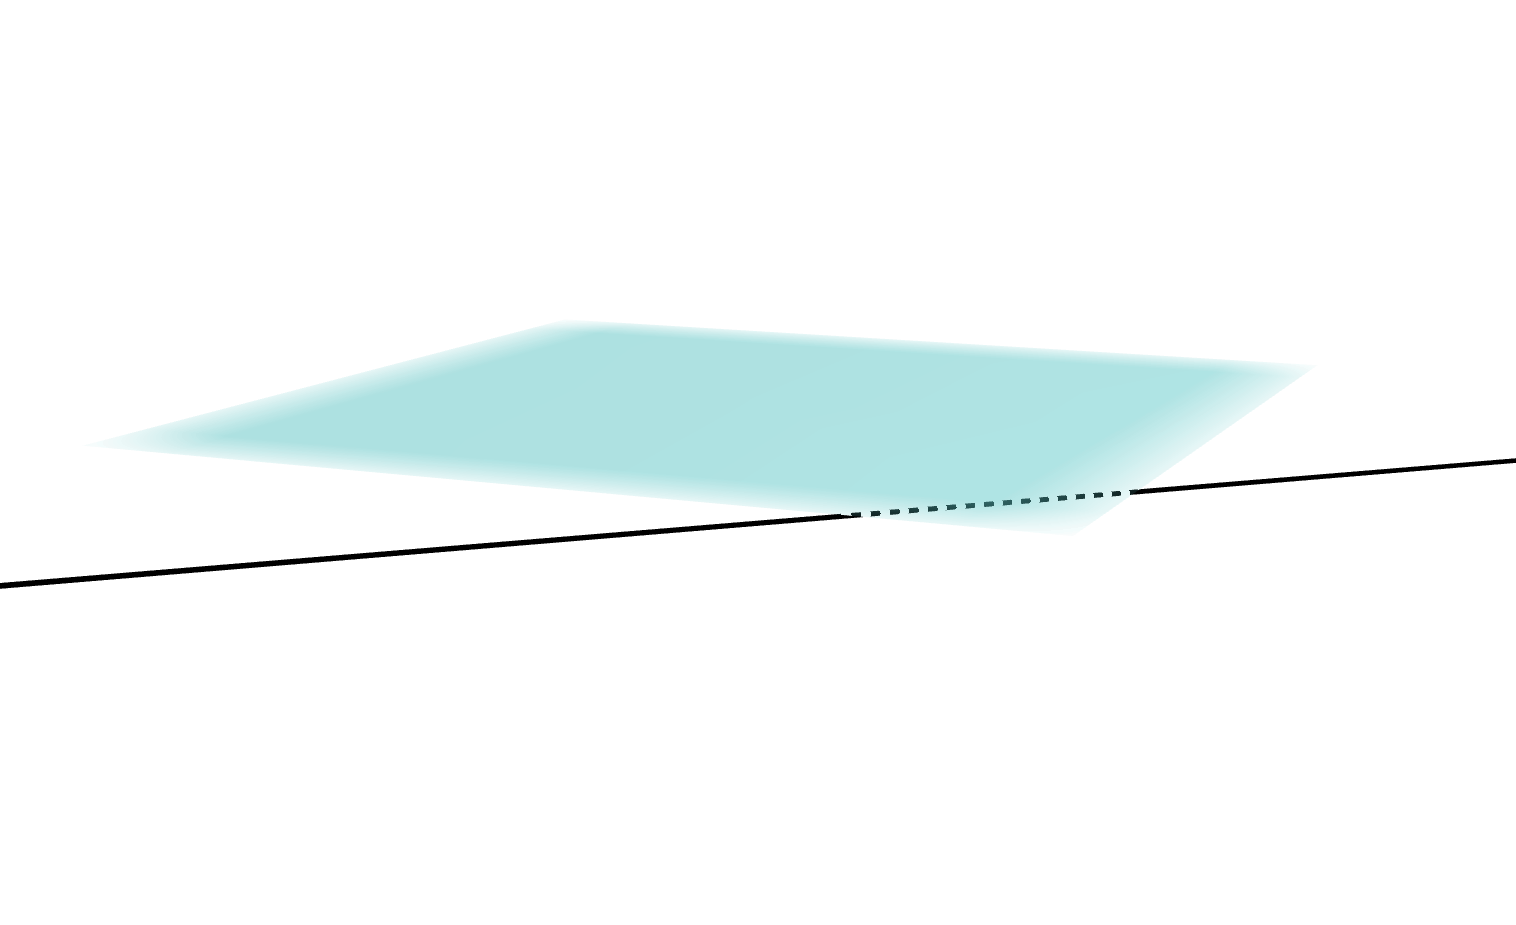
\includegraphics[width=4cm]{rsc/11fig5b.png}\\ \centering Droite strictement parallèle à un plan\end{minipage} % order of figures (b a c) intentional
                \begin{minipage}{4cm}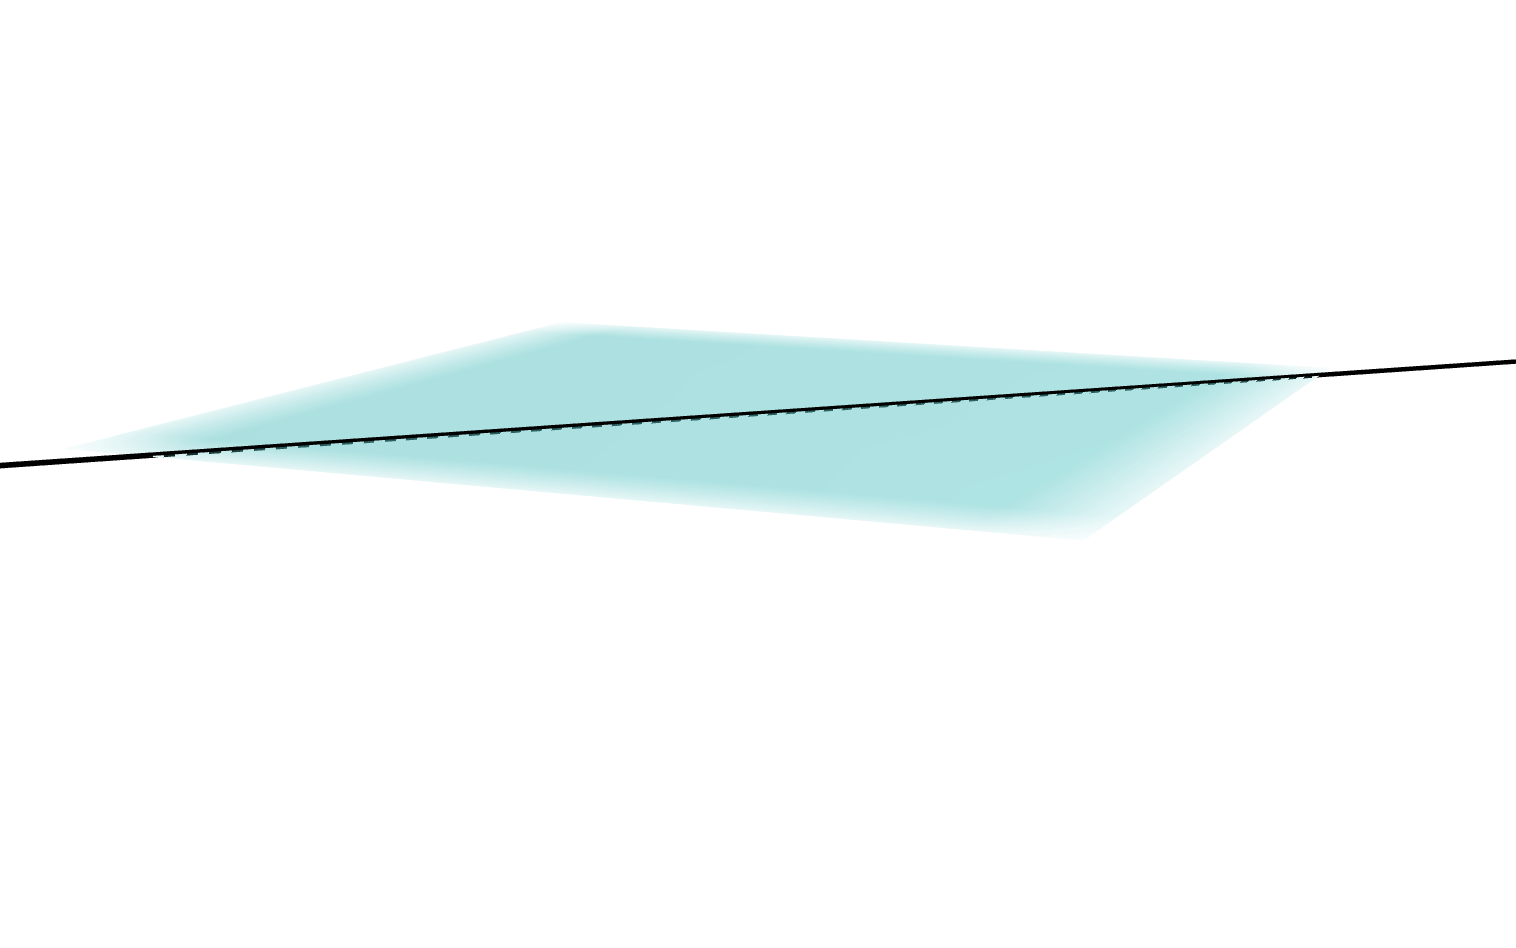
\includegraphics[width=4cm]{rsc/11fig5a.png}\\ \centering Droite incluse dans \\ un plan\end{minipage} 
                \begin{minipage}{4cm}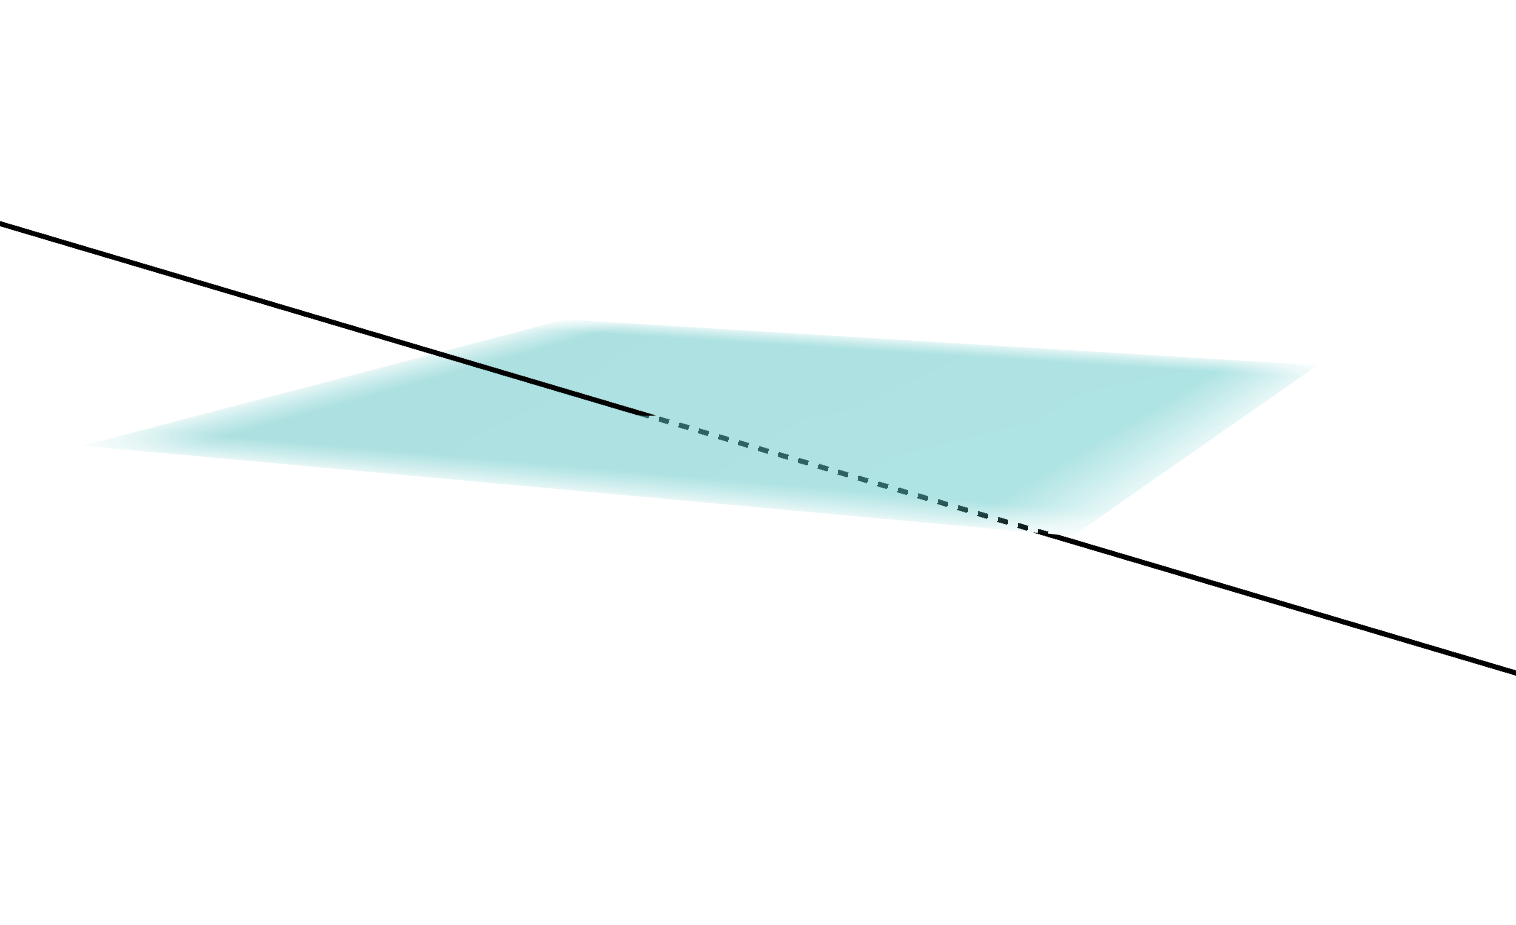
\includegraphics[width=4cm]{rsc/11fig5c.png}\\ \centering Droite sécante à un plan \end{minipage} \\[2ex]
                    C'est deux droites parallèles à un plan\hspace{4cm}\phantom{a} %shift text to left two only                
                \parbox{\linewidth}{\captionof{figure}{\centering Illustration des Positions Relatives d'un Plan et une Droite}}
            \end{center}
            \begin{SSpartie}{Propriété} 
                Une droite est parallèle à un plan si et seulement si elle est parallèle à une droite de ce plan.
            \end{SSpartie}
        \end{Spartie}
        \begin{Spartie}{Position Relative de Deux Droites} 
            \begin{SSpartie}{Définition} 
                Deux droites sont coplanaires si elles appartiennent à un même plan.
            \end{SSpartie}
            \begin{SSpartie}{Propriété} 
                Deux droites sont coplanaires si et seulement si elles sont sécantes ou parallèles.
                \begin{center}
                    \begin{minipage}{4cm}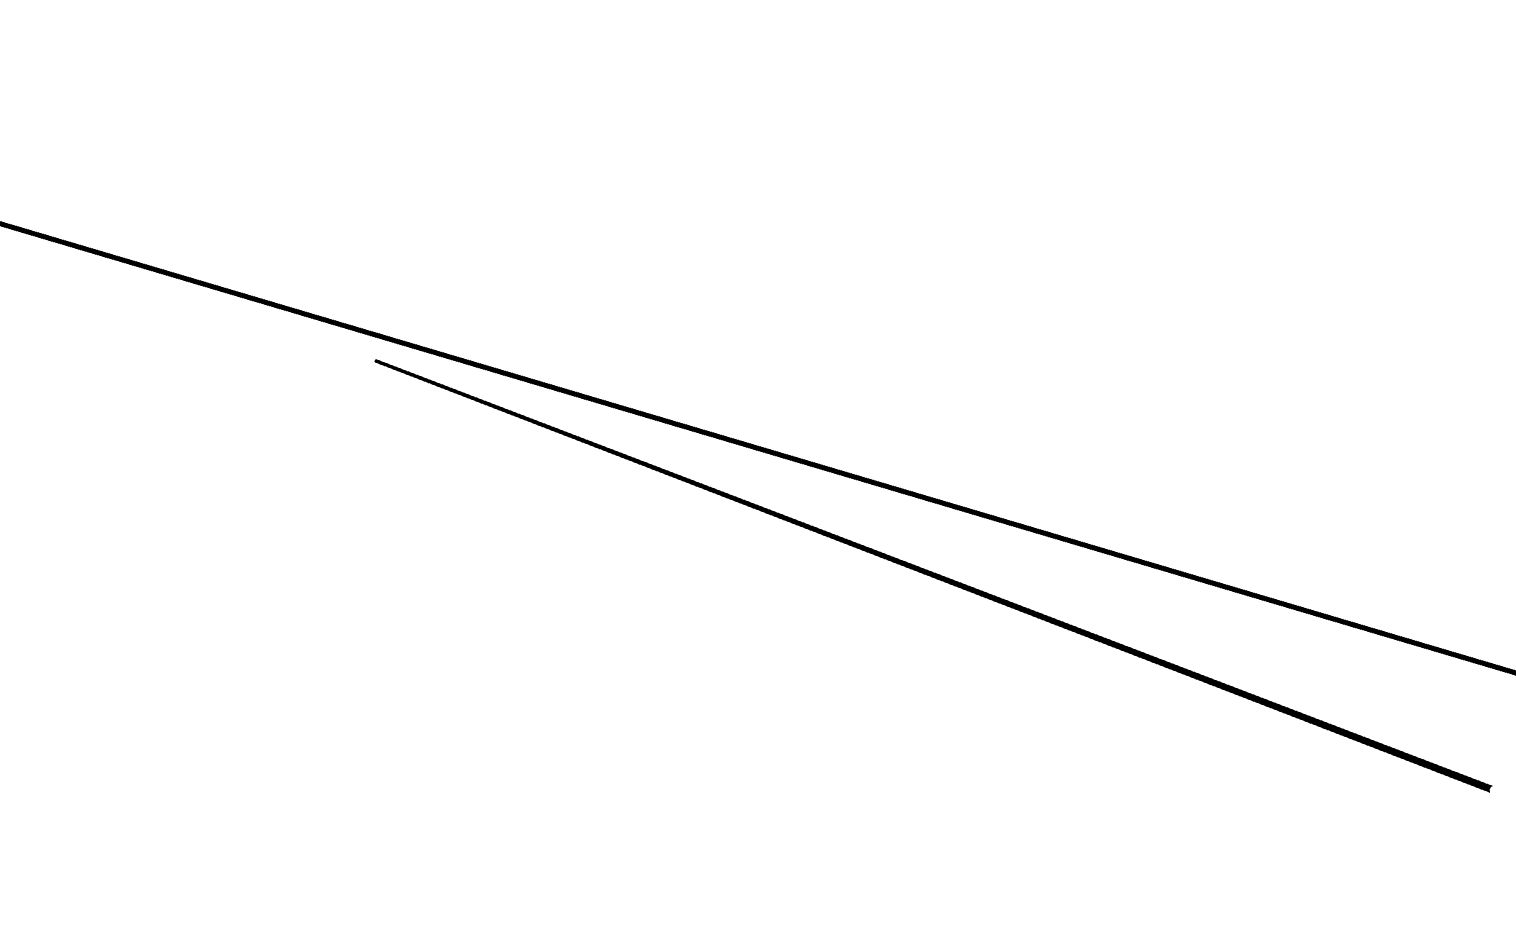
\includegraphics[width=4cm]{rsc/11fig6a.png}\\ \centering Droites non coplanaires\end{minipage}
                    \begin{minipage}{4cm}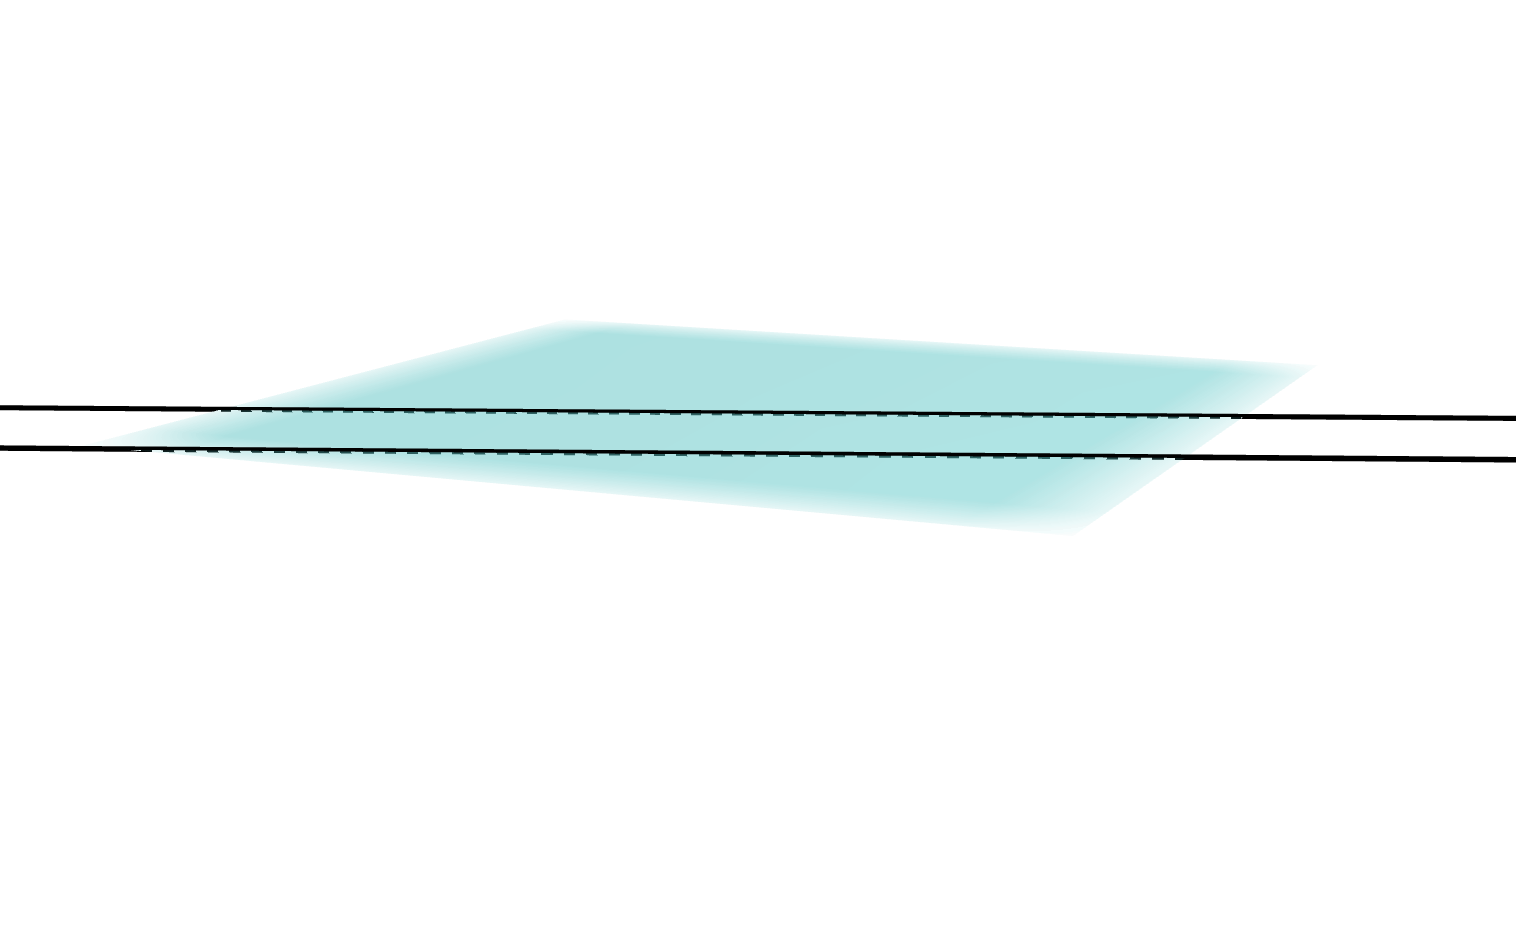
\includegraphics[width=4cm]{rsc/11fig6b.png}\\ \centering Droites strictement parallèles\end{minipage} 
                    \begin{minipage}{4cm}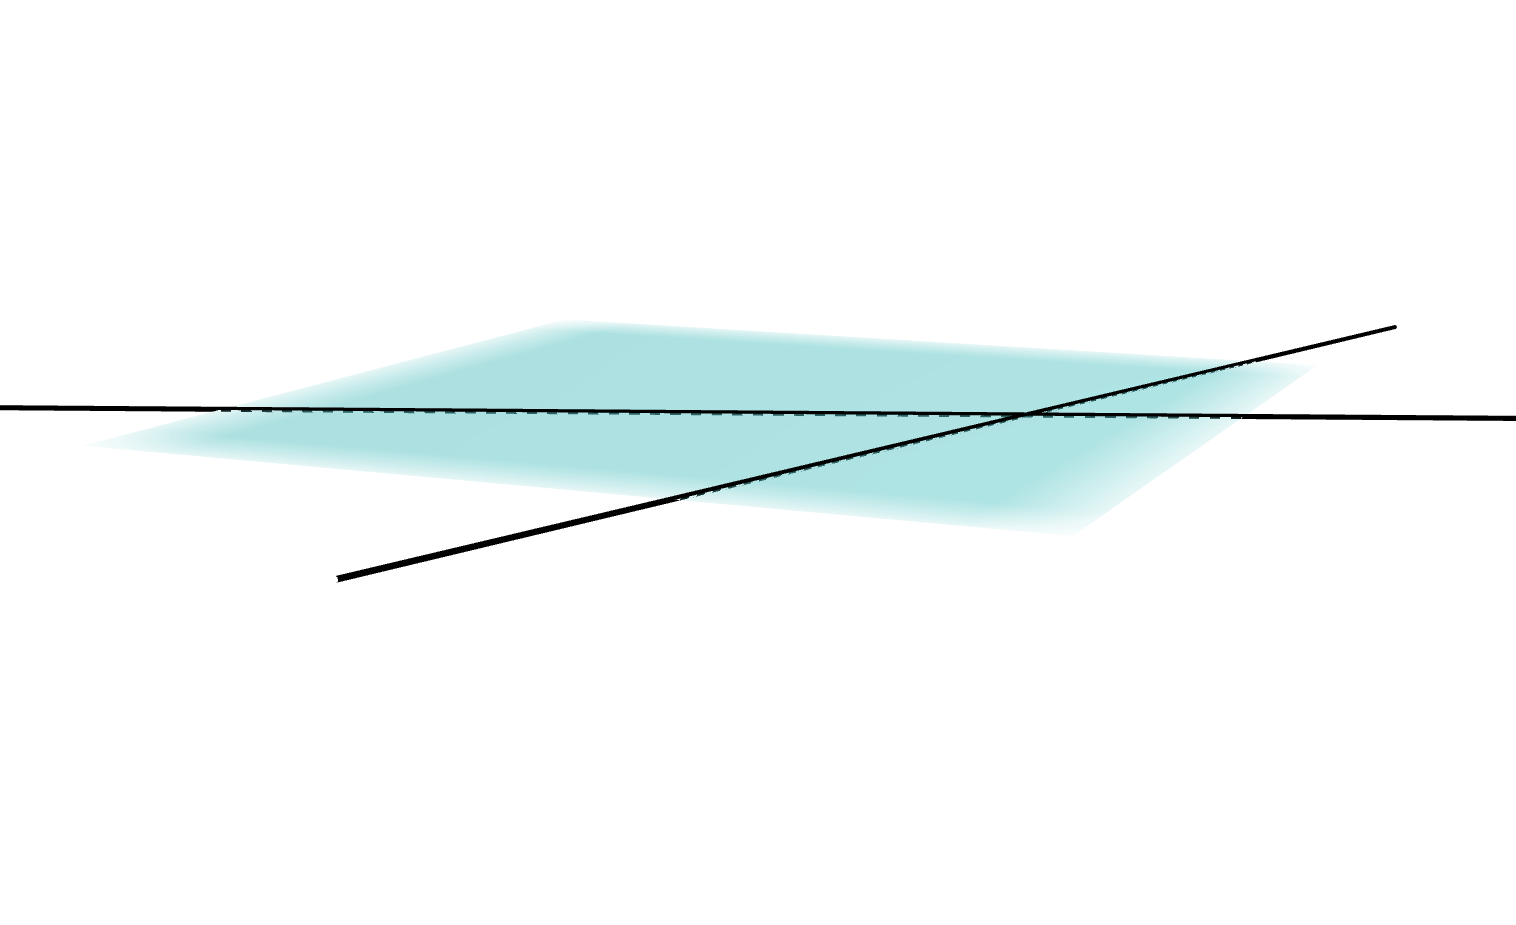
\includegraphics[width=4cm]{rsc/11fig6c.png}\\ \centering Droites sécantes\end{minipage}
                    \parbox{\linewidth}{\captionof{figure}{\centering Illustration de la Propriété}}
                \end{center}
            \end{SSpartie}
            \begin{SSpartie}{Remarque} 
                Deux droites confondues sont parallèles (au sens large)
            \end{SSpartie}
            \begin{SSpartie}{Remarque} 
                En général, deux droites de l'espace sont non coplanaires.
            \end{SSpartie}
        \end{Spartie}
    \end{Gpartie}
\end{document}